\documentclass{standalone}

\usepackage[dvipsnames]{xcolor}
\usepackage{pgfplots}
\usepackage{tikz}

\usepgfplotslibrary{statistics}

\begin{document}

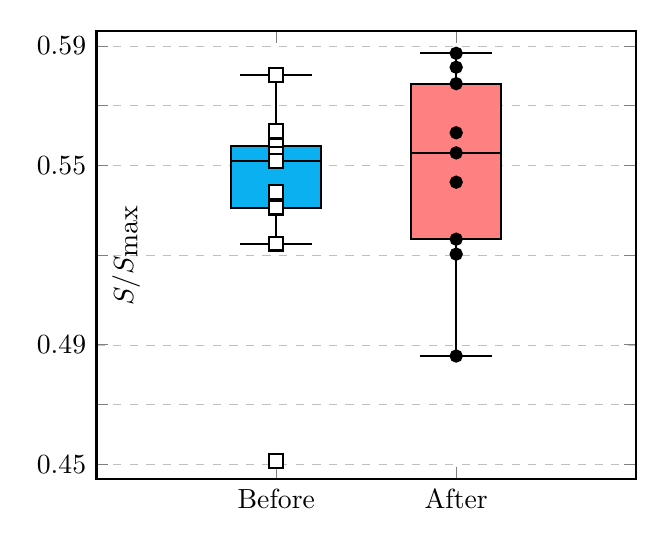
\begin{tikzpicture}

\begin{axis}[
	/pgfplots/boxplot/box extend=0.5,
	thick,
	xmin = 0, xmax = 3,
	ymax = 0.595, ymin = 0.445,
	xtick={1,2},
	ytick = {0.45, 0.47, 0.49, 0.52, 0.55, 0.57, 0.59},
	xticklabels={Before, After},
	yticklabels = {0.45, \,, 0.49, \,, 0.55, \,, 0.59},
	x label style={at={(axis description cs:0.5,0.0125)}},
	y label style={at={(axis description cs:0.1,.5)}},
	ylabel = $S/S_{\textrm{max}}$,
	ymajorgrids={true},
	grid style={dashed, line width=.1pt, draw=gray!50},
	boxplot/draw direction=y]

% ---------------------------------------------------------------
%                         "Before" Boxplot
% ---------------------------------------------------------------
	\addplot [
		thick,
		mark size = 1.5pt,
		boxplot,
		mark=*,
		fill = ProcessBlue,
		boxplot prepared={
			lower whisker=0.5238, 
			lower quartile=0.53585, % Q1
			median=0.55144,
			upper quartile=0.55639, % Q3
			upper whisker=0.58017,
			},
		] table [row sep=\\,y index=0] {
			0.45117\\ % outlier
	};

% ---------------------------------------------------------------
%                         "After" Boxplot
% ---------------------------------------------------------------
	\addplot [
		boxplot,
		thick,		
		mark=*,
		fill = red!50,
		boxplot prepared={
			lower whisker=0.48621,
			lower quartile=0.5253, % Q1
			median=0.55417,
			upper quartile=0.57734, % Q3
			upper whisker=0.5875,
			},
		] 
			% no outliers:
			coordinates {};


% ---------------------------------------------------------------
%                         Data points 
% ---------------------------------------------------------------
	\addplot[
	fill = white,
	mark = square*,
	mark size = 2.5pt,
	only marks
	] coordinates {
	( 1, 0.55639 )
	( 1, 0.56149 )
	( 1, 0.54105 )
	( 1, 0.53585 )
	( 1, 0.52380 )
	( 1, 0.45117 )
	( 1, 0.55283+0.001 ) % had to up its value for data viz...
	( 1, 0.55144 )
	( 1, 0.58017 )
	};

	\addplot[
	color = black,
	fill = black,
	mark = *,
	mark size = 2.0pt,
	only marks
	] coordinates {
	( 2, 0.52030 )
	( 2, 0.57734 )
	( 2, 0.55417 )
	( 2, 0.54437 )
	( 2, 0.56091 )
	( 2, 0.48621 )
	( 2, 0.58283 )
	( 2, 0.58750 )
	( 2, 0.52530 )
	};

% Outlier of the "Before" Boxplot
	\addplot[
		color = black,
		fill = white,
		mark = square*,
		mark size = 2.5pt,
		only marks
		] coordinates {
		( 1, 0.45117 )
		};
	
\end{axis}
\end{tikzpicture}

\end{document}
